\section{Overview of the FAIR facility}
The Facility of Antiproton and Ion Research in Europe (\gls{FAIR})~\cite{fair} is a future international research facility for accelerator-based research. 

\begin{figure}[!h]
    \centering
    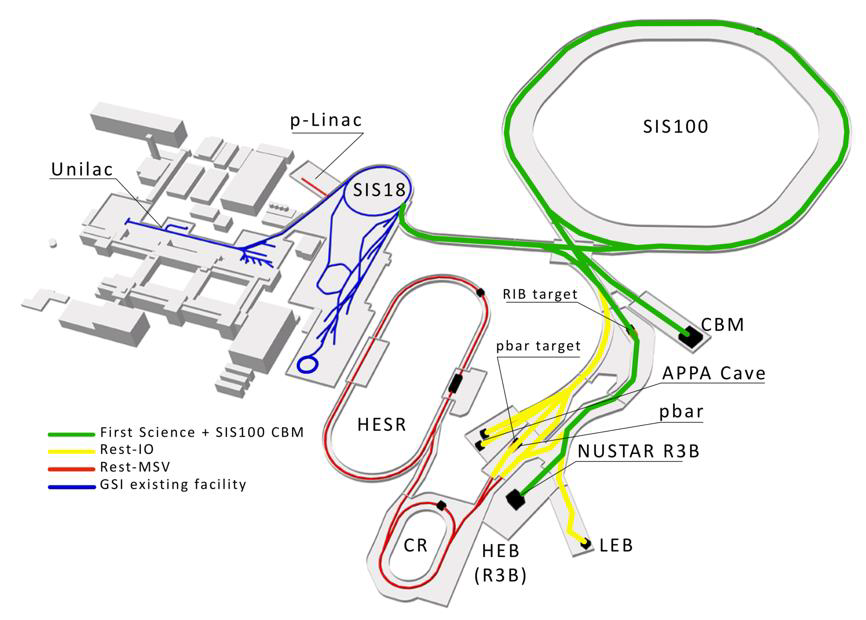
\includegraphics[width=0.85\columnwidth]{Chapter1/images/fair2.png}
    \caption{Overview of the GSI/FAIR research facility~\cite{fair}. The existing beamlines of the \gls{GSI} facility are denoted with blue lines. The planned facility and the corresponding experiments are located to the right.}
    \label{fig:fair}
\end{figure}

It will provide unique research opportunities in hadron and nuclear physics, atomic physics, nuclear astrophysics, materials research, plasma physics, and radiation biophysics, including developing novel medical treatments and applications for space science~\cite{fair1}. 
 
FAIR (see Figure \ref{fig:fair}) will extend GSI with Schwerionensynchrotron 100 (SIS100) accelerator, storage rings, and dedicated experiments from different fields, namely Atomic Physics, Plasma physics and Applications (APPA), antiProton ANnihilation at DArmstadt (PANDA), Nuclear Structure, Astrophysics, and Reactions (NUSTAR), and Compressed Baryonic Matter (\gls{CBM}). The latest status of SIS100 and its plans were recently described by Spiller~\cite{Spiller_2020}.

The SIS100, which will provide high-intensity beams of protons up
to energy of \gev{29}  with intensities up to $2.5\times 10^{13}$~protons/cycle and nuclei up to \agev{15} for Z/A = 0.5. Gold or uranium beams with kinetic energies up to \agev{11} will be available. Typical intensities for the heavy ions also depend on charge state and vary from 2.7~GeV/u for $\mathrm{U^{28+}}$ ions with $5\times 10^{11}$~ions/cycle to 10~GeV/u for $\mathrm{U^{92+}}$ ions with $4\times 10^{10}$~ions/cycle. High-intensity secondary beams will be produced by a large acceptance Superconducting Fragment Separator, which investigates very efficiently rare isotopes created in reactions with the primary beams. 

Moreover, a secondary antiproton beam will be produced by bombarding a metal target with 27.5 GeV protons. The collection of the pbar will be achieved with the \footnote{Magnetic horn is a high-current, pulsed focusing device used for the antiproton beam.}{magnetic horn}. The separation of the antiprotons from primary protons
and other secondary particles will be provided by the succeeding pbar separator, which will transfer antiprotons to the collector ring CR~\cite{SI100_CR}.

